
\serie{Points, segments et droites}

\begin{exercice}[Avec un quadrillage]
 \begin{center} 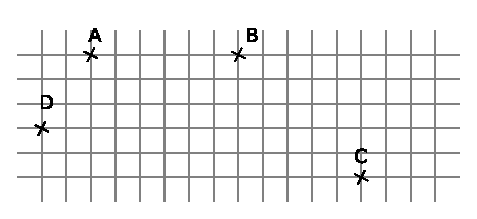
\includegraphics[width=7.2cm]{quadrillage} \end{center}
 \begin{enumerate}
  \item En utilisant le quadrillage de ton cahier, place les points $A$, $B$, $C$ et $D$ comme sur la figure ci-dessus :
  \item Trace en bleu le segment $[AB]$ ;
  \item Trace en vert le segment d'extrémités $D$ et $C$ ;
  \item Trace en rouge la droite passant par $A$ et $C$ ;
  \item Trace en noir la demi-droite d'origine $D$ passant par $B$.
  \end{enumerate}
 \end{exercice}


\begin{exercice}[Appartient ou pas ?]
 \begin{center} \includegraphics[width=4.8cm]{droiteABECD} \end{center}
 Après avoir observé la figure, recopie et complète les pointillés avec $\in$ ou $\notin$ :
    \begin{colenumerate}{3}
     \item $B$ \ldots $[AC]$ ;
     \item $D$ \ldots $[AB]$ ;
     \item $E$ \ldots $[AD]$ ;
     \item $B$ \ldots $[CA)$ ;
     \item $D$ \ldots $[CA)$ ;
     \item $E$ \ldots $[CE]$.
     \end{colenumerate}
\end{exercice}


\begin{exercice}[À trouver]
 \begin{center} 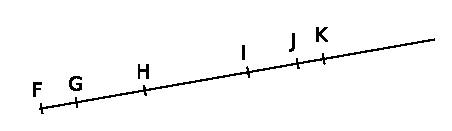
\includegraphics[width=6.5cm]{droiteFGHIJK}  \end{center}
 Parmi les points nommés sur la figure, indique ceux qui appartiennent à :
    \begin{colenumerate}{2}
     \item $[FK]$ ;
     \item $[IG)$ ;
     \item $[FJ]$ et à $[GK]$ ;
     \item $[GJ)$ mais pas à $[HJ]$ ;
     \item $[FG]$ ou à $[IJ)$ ;
     \item $[FH]$ et à $[JK]$.
     \end{colenumerate}
\end{exercice}


\begin{exercice}[Vrai ou faux ?]
 \begin{center} \includegraphics[width=4.6cm]{segmentsAB-CD}  \end{center}
 Observe cette figure composée de deux segments $[AB]$ et $[CD]$ sécants et indique pour chaque affirmation si elle est vraie ou fausse :
 \begin{enumerate}
  \item Les points $C$, $D$ et $M$ sont alignés ;
  \item $M$ est le point d'intersection de $[AB]$ et $[CD]$ ;
  \item $M$ est le milieu du segment $[AC]$ ;
  \item $M$ est un point du segment $[CD]$ ;
  \item $A$ appartient au segment $[MB]$ ;
  \item $M$ est le milieu du segment $[CD]$.
 \end{enumerate}
\end{exercice}


\begin{exercice}[Milieux]
\begin{enumerate} 
 \item Trace un segment $[RS]$ de longueur 4,8 cm et place son milieu $T$ ;
 \item Place un point $U$ qui ne soit pas aligné avec $R$ et $S$ ;
 \item Place le point $V$ tel que $T$ soit le milieu de $[UV]$.
 \end{enumerate}
\end{exercice}


\begin{exercice}[À construire]
\begin{enumerate} 
 \item Place trois points $A$, $B$ et $C$ non alignés ;
 \item Trace les segments $[BC]$ et $[AC]$ ;
 \item Marque le milieu $I$ du segment $[BC]$ et le milieu $J$ du segment $[AC]$ ;
 \item Trace le segment d'extrémités $B$ et $J$ ;
 \item Note $K$ le point d'intersection de $[AI]$ et $[BJ]$ ;
 \item Trace le segment $[AB]$ et place son milieu $L$. Trace enfin le segment $[CL]$. Que remarques‑tu ?
 \end{enumerate}
\end{exercice}


\begin{exercice}[À construire (bis)]
\begin{enumerate} 
 \item Place trois points $L$, $M$ et $N$ non alignés ;
 \item Place un point $A$ appartenant au segment $[LN]$ ;
 \item Place un point $B$ appartenant à la demi‑droite $[MN)$ mais n'appartenant pas au segment $[MN]$ ;
 \item Place le point $C$ aligné d'une part avec $A$ et $B$, et d'autre part avec $L$ et $M$.
 \end{enumerate}
\end{exercice}



%%%%%%%%%%%%%%%%%%%%Mise en page
\vspace{1em}
%%%%%%%%%%%%%%%%%%%%%%%%%%%%%%%



\begin{exercice}[Bande dessinée]
 \begin{center} 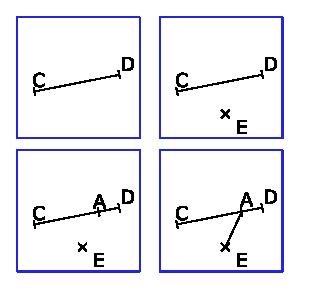
\includegraphics[width=4.3cm]{bande-dessinee}  \end{center}
Pour chaque étape de la bande dessinée, écris la consigne qui a été donnée, sans tenir compte des mesures.
\end{exercice}

%%%%%%%%%%%%%%%%%%%%%%%%%%%%%%%%%%%%%%%%%%%%%%%%%%%%%%%%%

\serie{Droites parallèles et perpendiculaires}

\begin{exercice}[Position de droites]
 \begin{center} \includegraphics[width=5.8cm]{mikado}  \end{center}
Observe la figure ci‑dessus et note sur ton cahier :
\begin{itemize}
 \item Le nom des droites qui \textbf{te semblent} perpendiculaires ;
 \item Le nom des droites qui sont sécantes mais non perpendiculaires ;
 \item Le nom des droites qui \textbf{te semblent} parallèles.
 \end{itemize}
\end{exercice}


\begin{exercice}[Position de droites (bis)]
 \begin{center} 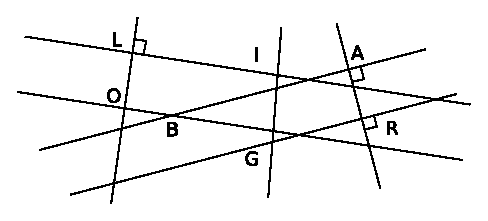
\includegraphics[width=7.3cm]{mikado2}  \end{center}
\begin{enumerate}
 \item Quelles sont les droites qui sont à coup sûr perpendiculaires ?
 \item Quelle semble être la position relative des droites $(BA)$ et $(GR)$ ?
 \end{enumerate}
\end{exercice}


\begin{exercice}[Quadrillage]
Reproduis une figure similaire à celle ci‑dessous. Trace, à la règle, la droite $d_1$ perpendiculaire à la droite $d$ passant par le point $M$ et la droite $d_2$ parallèle à la droite $d'$ passant par $M$.
\begin{center} \includegraphics[width=5.2cm]{quadrillage2}  \end{center}
\end{exercice}


\begin{exercice}[Constructions]
\begin{enumerate}
 \item Reproduis sur une feuille blanche les deux figures ci‑dessous :
 \begin{center} \includegraphics[width=6.1cm]{constructions}  \end{center}
 \item Pour chacune des figures, trace :
  \begin{itemize}
   \item La droite $d'$ perpendiculaire à $d$ et passant par $B$ ;
   \item La droite $d''$ perpendiculaire à $d$ et passant par $A$.
   \end{itemize}
 \item Que peux‑tu dire des droites $d'$ et $d''$ ?
 \end{enumerate}
\end{exercice}


\begin{exercice}[Constructions (bis)]
 \begin{center} \includegraphics[width=5.7cm]{constructions2}  \end{center}
\begin{enumerate}
 \item Reproduis la figure ci‑dessus ;
 \item Trace $d'$, la parallèle à $d$ passant par $A$ ;
 \item Trace $d''$, la parallèle à $d$ passant par $B$ ;
 \item Que peux‑tu dire des droites $d'$ et $d''$ ?
 \end{enumerate}
\end{exercice}


%%%%%%%%%%%%%%%%%%%%Mise en page
\newpage
%%%%%%%%%%%%%%%%%%%%%%%%%%%%%%%



\begin{exercice}[Programme de construction]
\begin{enumerate}
 \item Place deux points $A$ et $B$ tels que $AB = 8$ cm ;
 \item Place un point $L$ sur $[AB]$ tel que $AL = 3$ cm ;
 \item Trace la droite $d$ telle que $L \in d$ et $(AB) \perp d$ ;
 \item Place un point $C$ tel que $C \in d$ et $LC = 2$ cm ;
 \item Trace la droite $d'$ telle que $d' \parallel (AB)$ et $C \in d'$ ;
 \item Sur la demi‑droite $[BC)$, place le point $I$ tel que $BI = 7$ cm ;
 \item Trace la droite $d''$ telle que $I \in d''$ et $d'' \parallel (AC)$.
 \end{enumerate}
\end{exercice}


\begin{exercice}
Construis la figure suivante : \\[0.75em]
\begin{minipage}[c]{0.2\textwidth}
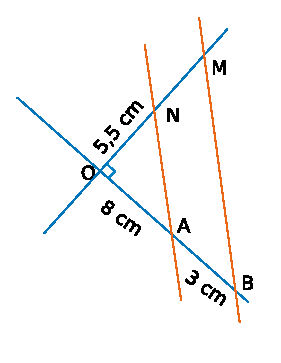
\includegraphics[width=3.8cm]{constructions3}
 \end{minipage} \hfill%
 \begin{minipage}[c]{0.2\textwidth}
 $(BM) \parallel (AN)$
  \end{minipage} \\
\end{exercice}


\begin{exercice}
Reproduis la figure ci‑dessous en vraie grandeur : \\[0.75em]
\begin{minipage}[c]{0.3\textwidth}
\includegraphics[width=4.5cm]{double-triangle}
 \end{minipage} \hfill%
 \begin{minipage}[c]{0.4\textwidth}
$AB = 5,3$ cm ;

$BC = 3$ cm ;

$AC = 7,7$ cm.
 \end{minipage} \\
\end{exercice}

%%%%%%%%%%%%%%%%%%%%%%%%%%%%%%%%%%%%%%%%%%%%%%%%%%%%%%%%%

\serie{Médiatrice d’un segment}

\begin{exercice}[Médiatrices]
Dans chaque cas, trace le segment de longueur donnée puis sa médiatrice :
 \begin{colenumerate}{3}
  \item $AB = 2$ cm ;
  \item $DE = 7,8$ cm ;
  \item $FG = 76$ mm.
  \end{colenumerate}
\end{exercice}


\begin{exercice}[Points alignés]
 \begin{enumerate}
  \item Trace un segment $[AB]$ de longueur 7 cm ;
  \item Place le point $C$ de la demi‑droite $[BA)$ tel que $BC = 12$ cm ;
  \item Construis la médiatrice $m_1$ du segment $[AC]$ ;
  \item Construis la médiatrice $m_2$ du segment $[AB]$ ;
  \item Que remarques‑tu ?
  \end{enumerate}
\end{exercice}


\begin{exercice}[Reconnaître]
Sur chacune des figures ci‑dessous, indique si $P$ est sur la médiatrice de $[AB]$ : \\[0.5em]
 \begin{colenumerate}{2}
  \item 
  
  \includegraphics[width=2.2cm]{mediatriceAB1}
  \item 
  
  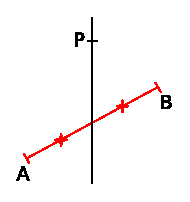
\includegraphics[width=2.2cm]{mediatriceAB2}
  \item 
  
  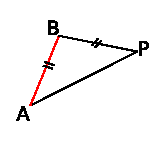
\includegraphics[width=2.2cm]{mediatriceAB3}
  \item 
  
  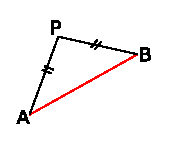
\includegraphics[width=2.2cm]{mediatriceAB4}
  \end{colenumerate}
\end{exercice}
 
 
\begin{exercice}[Construction]
 \begin{enumerate}
 \item Trace un segment $[AB]$ de longueur 6 cm ;
 \item Construis la médiatrice $d$ du segment $[AB]$ au compas ;
 \item Place un point $M$ sur $d$ à 7 cm de $A$ ;
 \item Quelle est la longueur de $[BM]$ ? 
 
Tu la justifieras en utilisant une propriété.
  \end{enumerate}
\end{exercice}


\begin{exercice}[Concours de médiatrices]
 \begin{enumerate}
 \item Place trois points $A$, $B$ et $C$ non alignés ;
 \item Trace sans équerre les médiatrices des segments $[AB]$, $[AC]$ et $[BC]$. 
 
 Que constates‑tu ?
 \end{enumerate}
\end{exercice}


%%%%%%%%%%%%%%%%%%%%Mise en page
\newpage
%%%%%%%%%%%%%%%%%%%%%%%%%%%%%%%



%%%%%%%%%%%%%%%%%%%%%%%%%%%%%%%%%%%%%%%%%%%%%%%%%%%%%%%%%

\serie{Nommer un angle}


\begin{exercice}[De toutes les couleurs]
Les points $A$, $O$ et $L$ sont alignés.
 \begin{center} 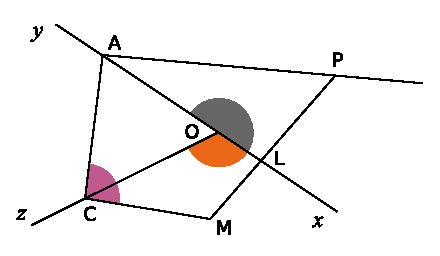
\includegraphics[width=6.7cm]{angles-colores}  \end{center}
\begin{enumerate}
 \item Nomme les angles marqués en couleur dans la figure de toutes les façons possibles ; 
 \item Reproduis la figure puis marque en bleu l'angle $\widehat{yOz}$, en rouge l'angle $\widehat{PMC}$ et en vert l'angle $\widehat{PAL}$.
 \end{enumerate}
\end{exercice}


\begin{exercice}[Plusieurs noms]
Les segments $[TD]$ et $[PS]$ sont sécants en $A$ et les segments $[PI]$ et $[TD]$ se coupent en $R$.

Trouve toutes les autres façons de nommer : \\[0.5em]
\begin{minipage}[c]{0.2\textwidth}
\begin{itemize}
 \item l'angle $\widehat{APR}$ ;
 \item l'angle $\widehat{RDI}$ ;
 \item l'angle $\widehat{PDA}$.
 \end{itemize}
 \end{minipage} \hfill%
  \begin{minipage}[c]{0.4\textwidth}
  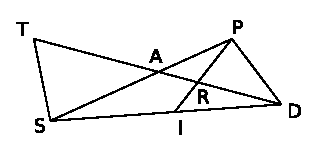
\includegraphics[width=4.7cm]{segments-secants}
  \end{minipage} \\
\end{exercice}  


\begin{exercice}[Quelle étourdie !]
Louise a recopié la figure ci‑dessous qui était au tableau mais elle a oublié de noter les noms des points d'intersection des droites. 
 \begin{center} 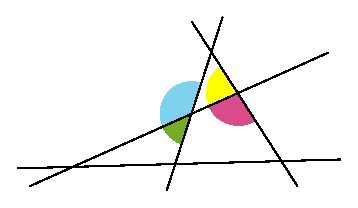
\includegraphics[width=5.2cm]{angles-multicolores}  \end{center}
Elle appelle son camarade Ahmed qui lui dit que les angles en couleur se nomment $\widehat{ABC}$, $\widehat{DBA}$, $\widehat{FAC}$ et $\widehat{FAE}$. \\[0.5em]
Reproduis la figure et nomme les points grâce à ces indications.
\end{exercice}  


%%%%%%%%%%%%%%%%%%%%Mise en page
\vspace{3em}
%%%%%%%%%%%%%%%%%%%%%%%%%%%%%%%




%%%%%%%%%%%%%%%%%%%%%%%%%%%%%%%%%%%%%%%%%%%%%%%%%%%%%%%%%

\serie{Mesure d'un angle}


\begin{exercice}[À vue d’œil]
Indique les angles qui te paraissent obtus, aigus ou droits.
 \begin{center} 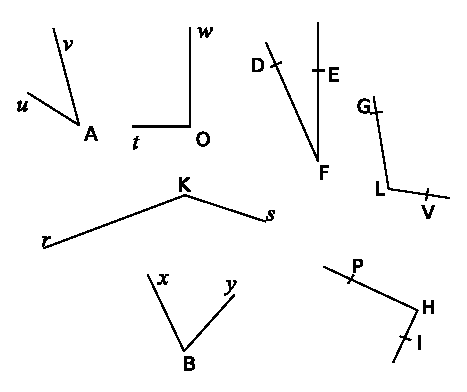
\includegraphics[width=7cm]{angles-toutgenre}  \end{center}
\end{exercice}


\begin{exercice}[Avec l'équerre]
En utilisant ton équerre, détermine quels sont les angles aigus, obtus ou droits dans chacun des cas ci-dessous.
 \begin{center} 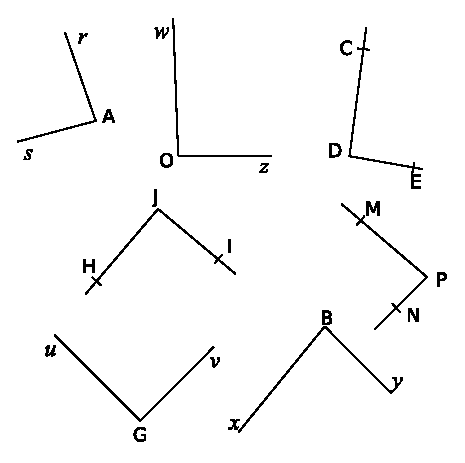
\includegraphics[width=7cm]{angles-droits}  \end{center}
\end{exercice}

%%%%%%%%%%%%%%%%%%%%Mise en page
\newpage
%%%%%%%%%%%%%%%%%%%%%%%%%%%%%%%

\begin{exercice}[Bien placé ?]
%Dans chacun des cas suivants, José souhaite mesurer l'angle $\widehat{BAC}$.

%Peut‑il effectuer une mesure correcte ? Si oui, indique la mesure de l'angle et si non, explique pourquoi. \\[0.5em]
\begin{colenumerate}{2}
%%%%%%%%%%%%%%%%%%%%%%%%%%%%%%%%%%%%%%%%%%%%%%%%%%%
%Rapporteur 1
%%%%%%%%%%%%%%%%%%%%%%%%%%%%%%%%%%%%%%%%%%%%%%%%%%%
 \item  %\includegraphics[width=3.6cm]{rapporteurA}

\scalebox{.8}{
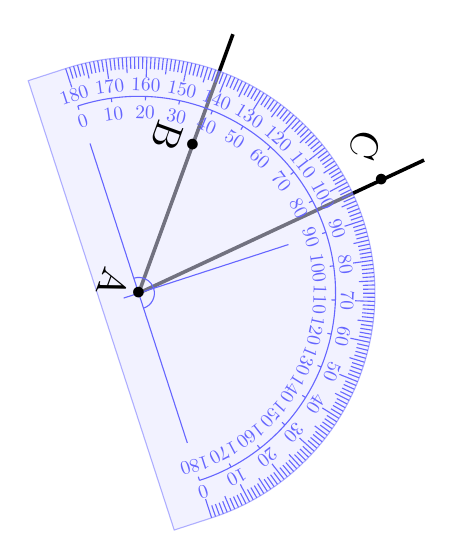
\begin{tikzpicture}

\def \RotFigure {-110} %rotation de toute la figure y compris textes
\begin{scope}[rotate=\RotFigure]

\def \CharSize {1.4};
\def \BulletSize {1};
\coordinate (A) at (0,0);
\coordinate (B) at (-2,0);
\coordinate (C) at (-2.404,2.404);
\coordinate (U) at (-3.5,0);
\coordinate (V) at (-2.828,2.828);

\draw[line width = 1.3pt] (U) -- (A) -- (V);
	
%début du rapporteur
    %Définition de l 'angle de rotation du rapporteur
    \def \RapRot {38} 
    %Définition du décalage du rapporteur
    \def \DecalX {0}
    \def \DecalY {0}
    %Couleur des élèments du rapporteur (sauf le remplissage)
    \def \RapColor {blue!60}
\begin{scope}[shift={(\DecalX,\DecalY)},rotate=\RapRot]
    % contours du rapporteur
    \draw[color=\RapColor, fill =blue!10, opacity=0.5] (-3,0) arc(180:0:3)--(3,-0.5)--(-3,-0.5)--cycle;	%Dont couleur de remplissage
    \draw[color=\RapColor] (-2,0)--(2,0);
    \draw[color=\RapColor] (0,-0.2)--(0,2);
    % graduation externe 1 degrés
    \foreach \a in {0,1,...,180}{\draw[color=\RapColor] (\a:3)--(\a:2.85);}
    % graduation externe 5 degrés
    \foreach \a in {0,5,...,180}{\draw[color=\RapColor] (\a:2.85)--(\a:2.8);}
    % double graduation
   \foreach \a/\b in {%
        0/-90,10/-80,20/-70,30/-60,40/-50,50/-40,%
        60/-30,70/-20,80/-10,90/0,100/10,110/20,%
        120/30,130/40,140/50,150/60,160/70,170/80,180/90%
    }{
    % graduation externe 10 degrés
    \draw[color=\RapColor] (\a:2.80)--(\a:2.75) 
    node[scale=0.7, rotate=\b+\RapRot+\RotFigure] (\a) at (\a:2.65){\a};
    % graduation interne 10 degrés
    \draw[color=\RapColor] (\a:2.5)--(\a:2.45)
	node[thin,scale=0.7, rotate=-\b+\RapRot+\RotFigure] (\a) at (180-\a:2.3){\a}; }
    % demi-cercle intérieur
    \draw[color=\RapColor](-2.5,0) arc(180:0:2.5);
    %demi-cercle à l'origine
    \draw[color=\RapColor](-0.2,0) arc(180:0:0.2);
\end{scope}
%fin du rapporteur

\draw (A) node [below,scale=\CharSize,rotate=\RotFigure]{A};
\draw (A) node[scale=\BulletSize]{$\bullet$};
\draw (B) node [below,scale=\CharSize,rotate=\RotFigure]{B};
\draw (B) node[scale=\BulletSize]{$\bullet$};
\draw (C) node [below left,scale=\CharSize,rotate=\RotFigure]{C};
\draw (C) node[scale=\BulletSize]{$\bullet$};
\end{scope}
\end{tikzpicture}
}


\item  %\vspace{-2em} 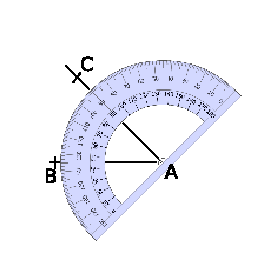
\includegraphics[width=3.6cm]{rapporteurB}
%%%%%%%%%%%%%%%%%%%%%%%%%%%%%%%%%%%%%%%%%%%%%%%%%%%
%Rapporteur 2
%%%%%%%%%%%%%%%%%%%%%%%%%%%%%%%%%%%%%%%%%%%%%%%%%%%

\scalebox{.8}{
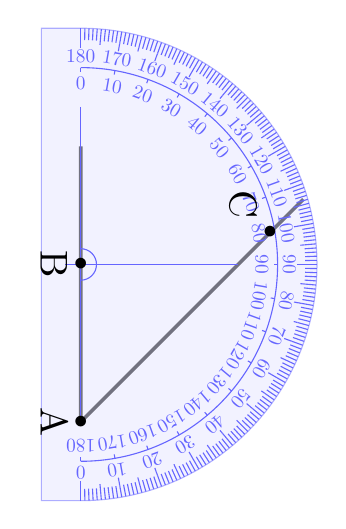
\begin{tikzpicture}

\def \RotFigure {-90} %rotation de toute la figure y compris textes
\begin{scope}[rotate=\RotFigure]

\def \CharSize {1.4};
\def \BulletSize {1};
\coordinate (A) at (0,0);
\coordinate (B) at (-2,0);
\coordinate (C) at (-2.404,2.404);
\coordinate (U) at (-3.5,0);
\coordinate (V) at (-2.828,2.828);

\draw[line width = 1.3pt] (U) -- (A) -- (V);
	
%début du rapporteur

    %Définition de l 'angle de rotation du rapporteur
    \def \RapRot {0} 
    %Définition du décalage du rapporteur
    \def \DecalX {-2}
    \def \DecalY {0}
    %Couleur des élèments du rapporteur (sauf le remplissage)
    \def \RapColor {blue!60}

\begin{scope}[shift={(\DecalX,\DecalY)},rotate=\RapRot]
    % contours du rapporteur
    \draw[color=\RapColor, fill =blue!10, opacity=0.5] (-3,0) arc(180:0:3)--(3,-0.5)--(-3,-0.5)--cycle;	%Dont couleur de remplissage
    \draw[color=\RapColor] (-2,0)--(2,0);
    \draw[color=\RapColor] (0,-0.2)--(0,2);
    % graduation externe 1 degrés
    \foreach \a in {0,1,...,180}{\draw[color=\RapColor] (\a:3)--(\a:2.85);}
    % graduation externe 5 degrés
    \foreach \a in {0,5,...,180}{\draw[color=\RapColor] (\a:2.85)--(\a:2.8);}
    % double graduation
   \foreach \a/\b in {%
        0/-90,10/-80,20/-70,30/-60,40/-50,50/-40,%
        60/-30,70/-20,80/-10,90/0,100/10,110/20,%
        120/30,130/40,140/50,150/60,160/70,170/80,180/90%
    }{
    % graduation externe 10 degrés
    \draw[color=\RapColor] (\a:2.80)--(\a:2.75) 
    node[scale=0.7, rotate=\b+\RapRot+\RotFigure] (\a) at (\a:2.65){\a};
    % graduation interne 10 degrés
    \draw[color=\RapColor] (\a:2.5)--(\a:2.45)
	node[thin,scale=0.7, rotate=-\b+\RapRot+\RotFigure] (\a) at (180-\a:2.3){\a}; }
    % demi-cercle intérieur
    \draw[color=\RapColor](-2.5,0) arc(180:0:2.5);
    %demi-cercle à l'origine
    \draw[color=\RapColor](-0.2,0) arc(180:0:0.2);
\end{scope}
%fin du rapporteur

\draw (A) node [below,scale=\CharSize,rotate=\RotFigure]{A};
\draw (A) node[scale=\BulletSize]{$\bullet$};
\draw (B) node [below,scale=\CharSize,rotate=\RotFigure]{B};
\draw (B) node[scale=\BulletSize]{$\bullet$};
\draw (C) node [below left,scale=\CharSize,rotate=\RotFigure]{C};
\draw (C) node[scale=\BulletSize]{$\bullet$};
\end{scope}
\end{tikzpicture}
}

 \item %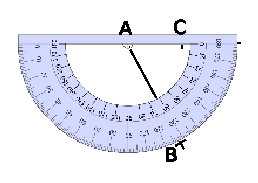
\includegraphics[width=3.6cm]{rapporteurC}
%%%%%%%%%%%%%%%%%%%%%%%%%%%%%%%%%%%%%%%%%%%%%%%%%%%
%Rapporteur 3
%%%%%%%%%%%%%%%%%%%%%%%%%%%%%%%%%%%%%%%%%%%%%%%%%%%

\scalebox{.8}{
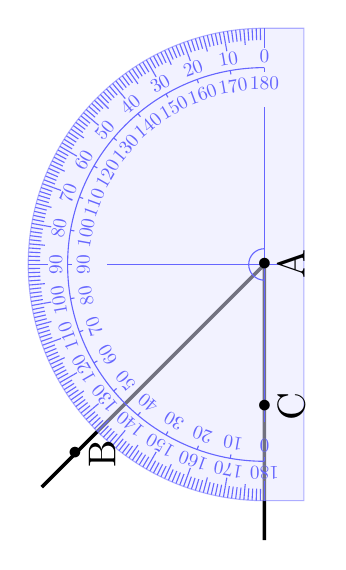
\begin{tikzpicture}

\def \RotFigure {-90} %rotation de toute la figure y compris textes
\begin{scope}[rotate=\RotFigure]

\def \CharSize {1.4};
\def \BulletSize {1};
\coordinate (A) at (0,0);
\coordinate (B) at (2.404,-2.404);
\coordinate (C) at (1.8,0);
\coordinate (U) at (3.5,0);
\coordinate (V) at (2.828,-2.828);

\draw[line width = 1.3pt] (U) -- (A) -- (V);
	
%début du rapporteur
    %Définition de l 'angle de rotation du rapporteur
    \def \RapRot {180} 
    %Définition du décalage du rapporteur
    \def \DecalX {0}
    \def \DecalY {0}
    %Couleur des élèments du rapporteur (sauf le remplissage)
    \def \RapColor {blue!60}

\begin{scope}[shift={(\DecalX,\DecalY)},rotate=\RapRot]
    % contours du rapporteur
    \draw[color=\RapColor, fill =blue!10, opacity=0.5] (-3,0) arc(180:0:3)--(3,-0.5)--(-3,-0.5)--cycle;	%Dont couleur de remplissage
    \draw[color=\RapColor] (-2,0)--(2,0);
    \draw[color=\RapColor] (0,-0.2)--(0,2);
    % graduation externe 1 degrés
    \foreach \a in {0,1,...,180}{\draw[color=\RapColor] (\a:3)--(\a:2.85);}
    % graduation externe 5 degrés
    \foreach \a in {0,5,...,180}{\draw[color=\RapColor] (\a:2.85)--(\a:2.8);}
    % double graduation
   \foreach \a/\b in {%
        0/-90,10/-80,20/-70,30/-60,40/-50,50/-40,%
        60/-30,70/-20,80/-10,90/0,100/10,110/20,%
        120/30,130/40,140/50,150/60,160/70,170/80,180/90%
    }{
    % graduation externe 10 degrés
    \draw[color=\RapColor] (\a:2.80)--(\a:2.75) 
    node[scale=0.7, rotate=\b+\RapRot+\RotFigure] (\a) at (\a:2.65){\a};
    % graduation interne 10 degrés
    \draw[color=\RapColor] (\a:2.5)--(\a:2.45)
	node[thin,scale=0.7, rotate=-\b+\RapRot+\RotFigure] (\a) at (180-\a:2.3){\a}; }
    % demi-cercle intérieur
    \draw[color=\RapColor](-2.5,0) arc(180:0:2.5);
    %demi-cercle à l'origine
    \draw[color=\RapColor](-0.2,0) arc(180:0:0.2);
\end{scope}
%fin du rapporteur

\draw (A) node [below,scale=\CharSize,rotate=-\RotFigure]{A};
\draw (A) node[scale=\BulletSize]{$\bullet$};
\draw (B) node [below,scale=\CharSize,rotate=-\RotFigure]{B};
\draw (B) node[scale=\BulletSize]{$\bullet$};
\draw (C) node [below,scale=\CharSize,rotate=-\RotFigure]{C};
\draw (C) node[scale=\BulletSize]{$\bullet$};
\end{scope}
\end{tikzpicture}
}

 \item  %\includegraphics[width=3.6cm]{rapporteurD}
%%%%%%%%%%%%%%%%%%%%%%%%%%%%%%%%%%%%%%%%%%%%%%%%%%%
%Rapporteur 4
%%%%%%%%%%%%%%%%%%%%%%%%%%%%%%%%%%%%%%%%%%%%%%%%%%%

\scalebox{.8}{
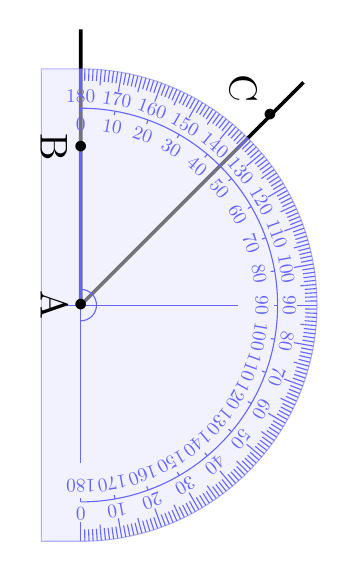
\begin{tikzpicture}

\def \RotFigure {-90} %rotation de toute la figure y compris textes
\begin{scope}[rotate=\RotFigure]

\def \CharSize {1.4};
\def \BulletSize {1};
\coordinate (A) at (0,0);
\coordinate (B) at (-2,0);
\coordinate (C) at (-2.404,2.404);
\coordinate (U) at (-3.5,0);
\coordinate (V) at (-2.828,2.828);

\draw[line width = 1.3pt] (U) -- (A) -- (V);
\draw (-0.5,0);
	
%début du rapporteur
    %Définition de l 'angle de rotation du rapporteur
    \def \RapRot {0} 
    %Définition du décalage du rapporteur
    \def \DecalX {0}
    \def \DecalY {0}
    %Couleur des élèments du rapporteur (sauf le remplissage)
    \def \RapColor {blue!60}

\begin{scope}[shift={(\DecalX,\DecalY)},rotate=\RapRot]
    % contours du rapporteur
    \draw[color=\RapColor, fill =blue!10, opacity=0.5] (-3,0) arc(180:0:3)--(3,-0.5)--(-3,-0.5)--cycle;	%Dont couleur de remplissage
    \draw[color=\RapColor] (-2,0)--(2,0);
    \draw[color=\RapColor] (0,-0.2)--(0,2);
    % graduation externe 1 degrés
    \foreach \a in {0,1,...,180}{\draw[color=\RapColor] (\a:3)--(\a:2.85);}
    % graduation externe 5 degrés
    \foreach \a in {0,5,...,180}{\draw[color=\RapColor] (\a:2.85)--(\a:2.8);}
    % double graduation
   \foreach \a/\b in {%
        0/-90,10/-80,20/-70,30/-60,40/-50,50/-40,%
        60/-30,70/-20,80/-10,90/0,100/10,110/20,%
        120/30,130/40,140/50,150/60,160/70,170/80,180/90%
    }{
    % graduation externe 10 degrés
    \draw[color=\RapColor] (\a:2.80)--(\a:2.75) 
    node[scale=0.7, rotate=\b+\RapRot+\RotFigure] (\a) at (\a:2.65){\a};
    % graduation interne 10 degrés
    \draw[color=\RapColor] (\a:2.5)--(\a:2.45)
	node[thin,scale=0.7, rotate=-\b+\RapRot+\RotFigure] (\a) at (180-\a:2.3){\a}; }
    % demi-cercle intérieur
    \draw[color=\RapColor](-2.5,0) arc(180:0:2.5);
    %demi-cercle à l'origine
    \draw[color=\RapColor](-0.2,0) arc(180:0:0.2);
\end{scope}
%fin du rapporteur

\draw (A) node [below,scale=\CharSize, rotate=\RotFigure]{A};
\draw (A) node[scale=\BulletSize]{$\bullet$};
\draw (B) node [below,scale=\CharSize, rotate=\RotFigure]{B};
\draw (B) node[scale=\BulletSize]{$\bullet$};
\draw (C) node [below left,scale=\CharSize, rotate=\RotFigure]{C};
\draw (C) node[scale=\BulletSize]{$\bullet$};
\end{scope}
\end{tikzpicture}
}
 
 \item % \includegraphics[width=3.6cm]{rapporteurD}
%%%%%%%%%%%%%%%%%%%%%%%%%%%%%%%%%%%%%%%%%%%%%%%%%%%
%Rapporteur 5
%%%%%%%%%%%%%%%%%%%%%%%%%%%%%%%%%%%%%%%%%%%%%%%%%%%



\scalebox{.8}{
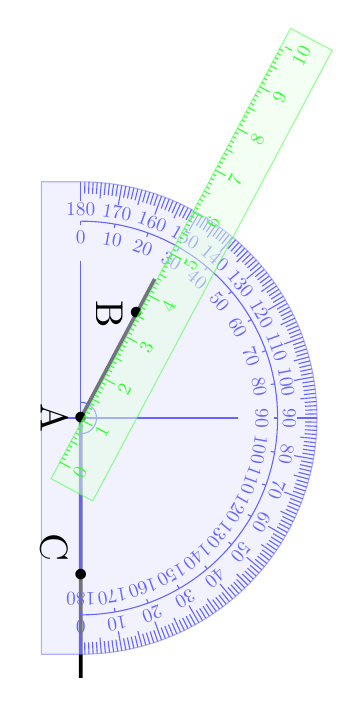
\begin{tikzpicture}

\def \RotFigure {-90} %rotation de toute la figure y compris textes
\begin{scope}[rotate=\RotFigure]

\def \CharSize {1.4};
\def \BulletSize {1};
\coordinate (A) at (0,0);
\coordinate (B) at (-1.324,0.704);
\coordinate (C) at (2,0);
\coordinate (U) at (-1.766,0.939);
\coordinate (V) at (3.3,0);

\draw[line width = 1.3pt] (U) -- (A) -- (V);
	
%début du rapporteur
    %Définition de l 'angle de rotation du rapporteur
    \def \Rotation {0} 
    %Définition du décalage du rapporteur
    \def \DecalX {0}
    \def \DecalY {0}
    %Couleur des élèments du rapporteur (sauf le remplissage)
    \def \RapColor {blue!60}

\begin{scope}[shift={(\DecalX,\DecalY)},rotate=\Rotation]
    % contours du rapporteur
    \draw[color=\RapColor, fill =blue!10, opacity=0.5] (-3,0) arc(180:0:3)--(3,-0.5)--(-3,-0.5)--cycle;	%Dont couleur de remplissage
    \draw[color=\RapColor] (-2,0)--(2,0);
    \draw[color=\RapColor] (0,-0.2)--(0,2);
    % graduation externe 1 degrés
    \foreach \a in {0,1,...,180}{\draw[color=\RapColor] (\a:3)--(\a:2.85);}
    % graduation externe 5 degrés
    \foreach \a in {0,5,...,180}{\draw[color=\RapColor] (\a:2.85)--(\a:2.8);}
    % double graduation
   \foreach \a/\b in {%
        0/-90,10/-80,20/-70,30/-60,40/-50,50/-40,%
        60/-30,70/-20,80/-10,90/0,100/10,110/20,%
        120/30,130/40,140/50,150/60,160/70,170/80,180/90%
    }{
    % graduation externe 10 degrés
    \draw[color=\RapColor] (\a:2.80)--(\a:2.75) 
    node[scale=0.7, rotate=\b+\Rotation+\RotFigure] (\a) at (\a:2.65){\a};
    % graduation interne 10 degrés
    \draw[color=\RapColor] (\a:2.5)--(\a:2.45)
	node[thin,scale=0.7, rotate=-\b+\Rotation+\RotFigure] (\a) at (180-\a:2.3){\a}; }
    % demi-cercle intérieur
    \draw[color=\RapColor](-2.5,0) arc(180:0:2.5);
    %demi-cercle à l'origine
    \draw[color=\RapColor](-0.2,0) arc(180:0:0.2);
\end{scope}
%fin du rapporteur

\draw (A) node [below,scale=\CharSize,rotate=\RotFigure]{A};
\draw (A) node[scale=\BulletSize]{$\bullet$};
\draw (B) node [below,scale=\CharSize,rotate=\RotFigure]{B};
\draw (B) node[scale=\BulletSize]{$\bullet$};
\draw (C) node [below left,scale=\CharSize,rotate=\RotFigure]{C};
\draw (C) node[scale=\BulletSize]{$\bullet$};

	
%début de la règle
    %Graduaton max. de la règle
    \def \TailleRegle {10}
    %Définition de l 'angle de rotation de la règle
    \def \RotationRegle {152}
    %Définition du décalage de la règle
    \def \DecalRegleX {0.7}
    \def \DecalRegleY {0}
    %Couleur des élèments de la règle (sauf le remplissage)
    \def \RegleColor {green!80}

\begin{scope}[shift={(\DecalRegleX,\DecalRegleY)},rotate=\RotationRegle, scale=0.6]
    % contours de la règle
    \draw[color=\RegleColor, fill =green!10, opacity=0.5] (-0.4,0.5) rectangle (\TailleRegle+0.4,-0.5);	%Dont couleur de remplissage
    % graduation 1 mm
    \foreach \a in {0,0.1,...,\TailleRegle}{\draw[color=\RegleColor] (\a,0.5)--(\a,0.42);}
    % graduation 5 mm
    \foreach \a in {0,0.5,...,\TailleRegle}{\draw[color=\RegleColor] (\a,0.42)--(\a,0.35);}
    % graduation et repères 10 mm
    \foreach \a in {0,1,...,\TailleRegle}{\draw[color=\RegleColor] (\a,0.35)--(\a,0.25)
    node[scale=0.7, rotate=\RotationRegle+\RotFigure] (\a) at (\a,0.02){\a};}
    
\end{scope}
%fin de la règle

\end{scope}
\end{tikzpicture}
}

 \item % \vspace{-2em} 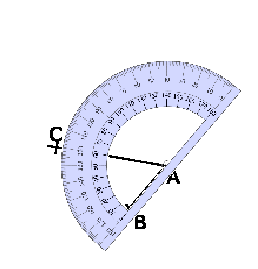
\includegraphics[width=3.6cm]{rapporteurF}
%%%%%%%%%%%%%%%%%%%%%%%%%%%%%%%%%%%%%%%%%%%%%%%%%%%
%Rapporteur 6
%%%%%%%%%%%%%%%%%%%%%%%%%%%%%%%%%%%%%%%%%%%%%%%%%%%

\scalebox{.8}{
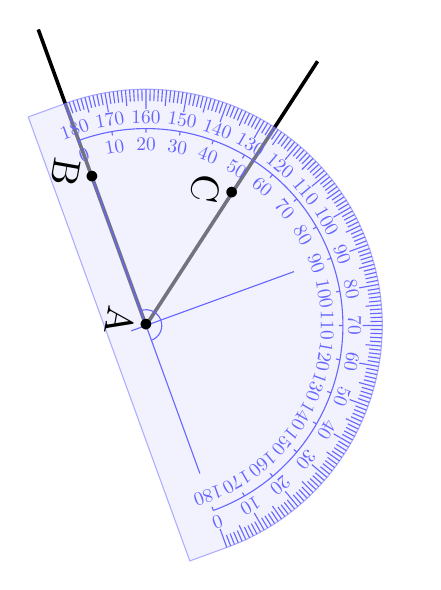
\begin{tikzpicture}

\def \RotFigure {-100} %rotation de toute la figure y compris textes
\begin{scope}[rotate=\RotFigure]

\def \CharSize {1.4};
\def \BulletSize {1};
\coordinate (A) at (0,0);
\coordinate (B) at (-1.732,-1);
\coordinate (C) at (-1.841,0.781);
\coordinate (U) at (-3.464,-2);
\coordinate (V) at (-3.682,1.563);

\draw[line width = 1.3pt] (U) -- (A) -- (V);

%début du rapporteur
    %Définition de l 'angle de rotation du rapporteur
    \def \RapRot {30} 
    %Définition du décalage du rapporteur
    \def \DecalX {0}
    \def \DecalY {0}
    %Couleur des élèments du rapporteur (sauf le remplissage)
    \def \RapColor {blue!60}

\begin{scope}[shift={(\DecalX,\DecalY)},rotate=\RapRot]

    % contours du rapporteur
    \draw[color=\RapColor, fill =blue!10, opacity=0.5] (-3,0) arc(180:0:3)--(3,-0.5)--(-3,-0.5)--cycle;	%Dont couleur de remplissage
    \draw[color=\RapColor] (-2,0)--(2,0);
    \draw[color=\RapColor] (0,-0.2)--(0,2);
    % graduation externe 1 degrés
    \foreach \a in {0,1,...,180}{\draw[color=\RapColor] (\a:3)--(\a:2.85);}
    % graduation externe 5 degrés
    \foreach \a in {0,5,...,180}{\draw[color=\RapColor] (\a:2.85)--(\a:2.8);}
    % double graduation
   \foreach \a/\b in {%
        0/-90,10/-80,20/-70,30/-60,40/-50,50/-40,%
        60/-30,70/-20,80/-10,90/0,100/10,110/20,%
        120/30,130/40,140/50,150/60,160/70,170/80,180/90%
    }{
    % graduation externe 10 degrés
    \draw[color=\RapColor] (\a:2.80)--(\a:2.75) 
    node[scale=0.7, rotate=\b+\RapRot+\RotFigure] (\a) at (\a:2.65){\a};
    % graduation interne 10 degrés
    \draw[color=\RapColor] (\a:2.5)--(\a:2.45)
	node[thin,scale=0.7, rotate=-\b+\RapRot+\RotFigure] (\a) at (180-\a:2.3){\a}; }
    % demi-cercle intérieur
    \draw[color=\RapColor](-2.5,0) arc(180:0:2.5);
    %demi-cercle à l'origine
    \draw[color=\RapColor](-0.2,0) arc(180:0:0.2);
\end{scope}
%fin du rapporteur

\draw (A) node [below,scale=\CharSize,rotate=\RotFigure]{A};
\draw (A) node[scale=\BulletSize]{$\bullet$};
\draw (B) node [below,scale=\CharSize,rotate=\RotFigure]{B};
\draw (B) node[scale=\BulletSize]{$\bullet$};
\draw (C) node [below,scale=\CharSize,rotate=\RotFigure]{C};
\draw (C) node[scale=\BulletSize]{$\bullet$};
\end{scope}
\end{tikzpicture}
}



 \end{colenumerate}

%%%%%%%%%%%%%%%%%%%%%%%%%%%%%%%%%%%%%

\phantom{Coucou}

%%%%%%%%%%%%%%%%%%%%%%%%%%%%%%%%%%%%%

\end{exercice}  


\begin{exercice}[Alignés ?]
Dans la figure ci-dessous faite à main levée, on donne : $\widehat{LIS}= 44^\circ$.
Les points $F$, $I$ et $L$ sont-ils alignés ? Justifie.
 \begin{center} 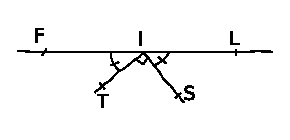
\includegraphics[width=4.2cm]{croquis-tordu} \end{center}
\end{exercice} 



\begin{exercice}[Quelle échelle ?]
Pour chaque angle, indique s'il est aigu ou obtus. Note ensuite sa mesure sur la bonne graduation du rapporteur.
\begin{colenumerate}{2}
 \item  
 
 \includegraphics[width=3.3cm]{rapporteur-bleu}
 \item 
 
 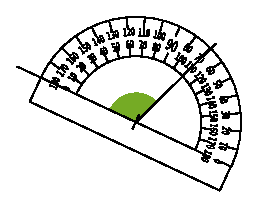
\includegraphics[width=3.2cm]{rapporteur-vert}
 \item 

 \includegraphics[width=3.1cm]{rapporteur-rose}
 \item 
 
 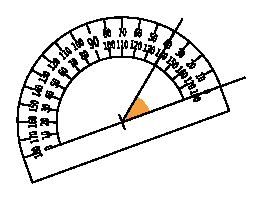
\includegraphics[width=3.3cm]{rapporteur-orange}
 
 \end{colenumerate}
\end{exercice} 

\begin{exercice}
Mesure les angles ci‑dessous avec ton rapporteur.
 \begin{center} 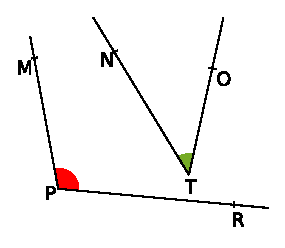
\includegraphics[width=4cm]{angles-rose-vert} \end{center}
 
 \begin{center} 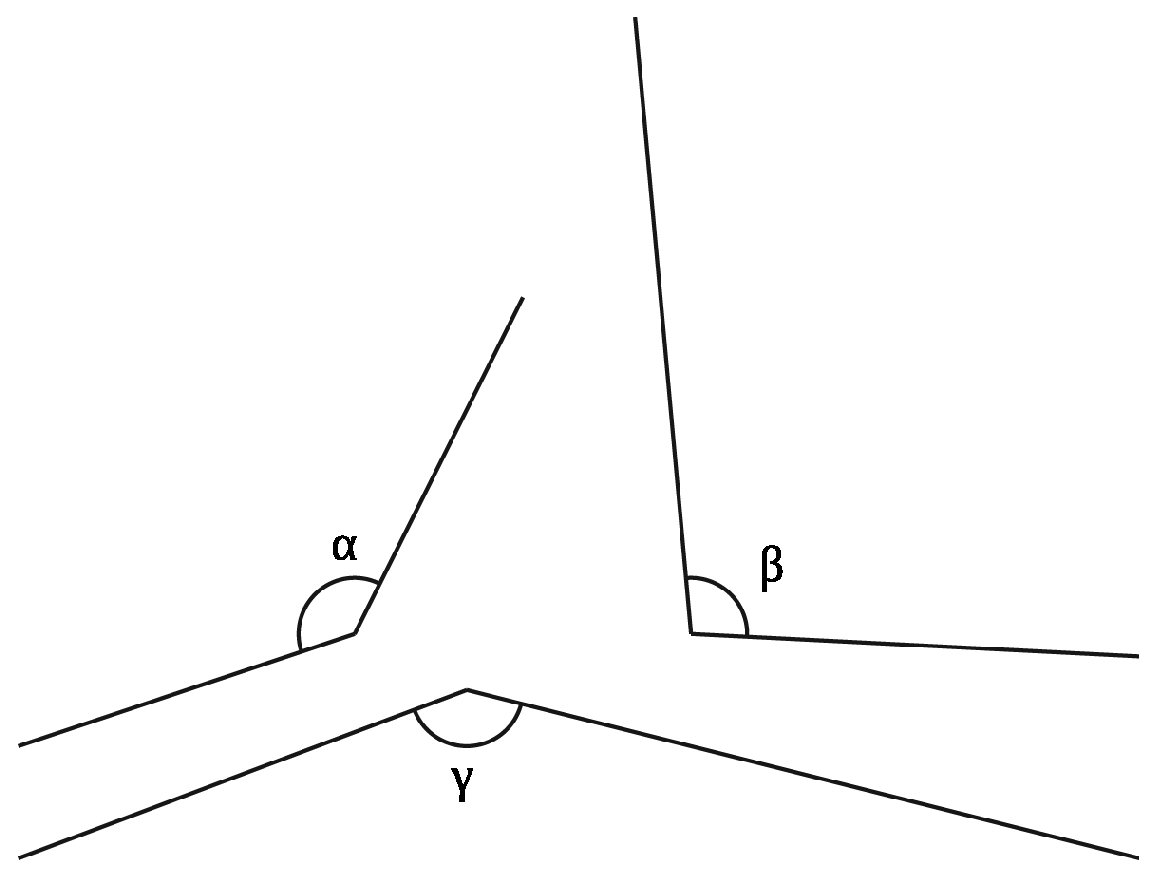
\includegraphics[width=4cm]{angles-gris} \end{center}
\end{exercice} 




%%%%%%%%%%%%%%%%%%%%Mise en page
\newpage
%%%%%%%%%%%%%%%%%%%%%%%%%%%%%%%



%%%%%%%%%%%%%%%%%%%%%%%%%%%%%%%%%%%%%%%%%%%%%%%%%%%%%%%%%

\serie{Construire un angle}

\begin{exercice}
Construis les angles suivants :

$\widehat{MOT} = 27^\circ$ ; $\widehat{SUD} = 151^\circ$ ; $\widehat{FIN} = 47^\circ$ et $\widehat{PRE} = 110^\circ$.
\end{exercice} 


\begin{exercice}[Programme de construction]
\begin{enumerate}
\item Trace $[AC]$ tel que $AC = 3$ cm. Construis un angle $\widehat{ACx}$ mesurant $60^\circ$. Place un point $B$ sur $[Cx)$ tel que $CB = 5,6$ cm ;
\item Place le point $D$ sur $[AB]$ tel que $\widehat{DCB} = 25^\circ$ ;
\item Place le point $E$ sur $[AD]$ tel que $\widehat{DCE} = 25^\circ$.
\end{enumerate}
\end{exercice} 


\begin{exercice}[Secteur angulaire]
Voici une figure construite par Joséphine. Reproduis la figure sur ton cahier.
 \begin{center} 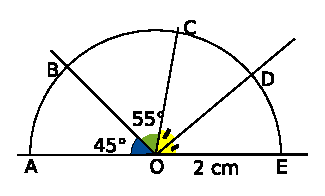
\includegraphics[width=4.7cm]{secteurABCDE} \end{center}
\end{exercice} 


\begin{exercice}[Reproduction de figure]
 \begin{center} 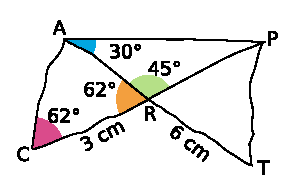
\includegraphics[width=4.2cm]{croquisAPCTR} \end{center}
 Voici le croquis d’une figure dans laquelle les points $A$, $R$ et $T$ sont alignés. Construis la figure.
\end{exercice} 


%%%%%%%%%%%%%%%%%%%%%%%%%%%%%%%%%%%Mise en page
\columnbreak
%%%%%%%%%%%%%%%%%%%%%%%%%%%%%%%%%%%%%%%%%%%%%%


%%%%%%%%%%%%%%%%%%%%%%%%%%%%%%%%%%%%%%%%%%%%%%%%%%%%%%%%%

\serie{Bissectrice d'un angle}

\begin{exercice}[Reconnaître]
Pour quelle(s) figure(s) la demi‑droite rouge semble être la bissectrice de l'angle ?
\begin{colenumerate}{3}
 \item  
 
 \includegraphics[width=1.2cm]{demidroite1}
 \item 
 
 \includegraphics[width=1.2cm]{demidroite2}
 \item 
 
 \includegraphics[width=1.2cm]{demidroite3}
 \item 
 
 \includegraphics[width=2cm]{demidroite4}
 \item
 
 \includegraphics[width=2cm]{demidroite5}

 \end{colenumerate}
\end{exercice} 


\begin{exercice}[Bissectrice et construction]
Dans chaque cas, trace un angle dont la mesure est donnée puis construis sa bissectrice au compas :
\begin{colenumerate}{3}
 \item $\widehat{ABC} = 32^\circ$ ;
  \item $\widehat{UST} = 180^\circ$ ; 
  \item $\widehat{ZXY} = 67^\circ$ ;
  \item $\widehat{WZD} = 90^\circ$ ;
  \item $\widehat{PRT} = 127^\circ$ ;
  \item $\widehat{LKI} = 154^\circ$.
 \end{colenumerate}
\end{exercice} 


\begin{exercice}[Mesure d'angles]
\begin{enumerate}
 \item Trace un angle $\widehat{EDF}$ qui mesure $28^\circ$ ; \label{PtSegDr_entrain_mesangl_a}
 \item Construis la bissectrice de $\widehat{EDF}$ et place un point $G$ sur celle‑ci ;
 \item Calcule la mesure de l'angle $\widehat{GDF}$. Justifie ; \label{PtSegDr_entrain_mesangl_c}
 \item Recommence les questions de \ref{PtSegDr_entrain_mesangl_a} à \ref{PtSegDr_entrain_mesangl_c} avec un angle de $133^\circ$.
 \end{enumerate}
\end{exercice} 


%%%%%%%%%%%%%%%%%%%%%%%%%%%%%%%%%%%Mise en page

\vspace*{3cm}

\phantom{coucou}

\pagebreak
%%%%%%%%%%%%%%%%%%%%%%%%%%%%%%%%%%%%%%%%%%%%%%


%%%%%%%%%%%%%%%%%%%%%%%%%%%%%%%%%%%%%%%%%%%%%%%%%%%%%%%%%

\serie{Cercle}

\begin{exercice}[Vocabulaire]
 \begin{center} 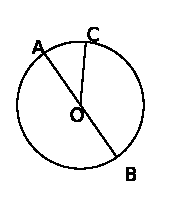
\includegraphics[width=1.9cm]{cercleABC} \end{center}
 Sur la figure ci-dessus : 
 
$A$, $B$ et $C$ sont sur le cercle de centre $O$ ;

$A$, $O$ et $B$ sont alignés.
 \begin{enumerate}
  \item Écris deux phrases décrivant la figure, en utilisant les mots « rayon » et « diamètre » ;
  \item Complète les phrases suivantes :
   \begin{itemize}
    \item Le point $O$ est le milieu du \dotfill ;
    \item Le point $O$ est une extrémité du \dotfill ;
    \item $A$ et $B$ sont les \dotfill du \dotfill $[AB]$ ;
    \item La portion de cercle comprise entre les points $A$ et $C$ est l'\dotfill.
    \end{itemize}
  \end{enumerate}
\end{exercice}


\begin{exercice}[Avec le rayon]
Trace un cercle de centre $O$ et de rayon 4 cm puis un cercle de rayon 4 cm et passant par $O$.
\end{exercice}


\begin{exercice}[Avec le diamètre]
 \begin{enumerate}
  \item Trace un segment $[AB]$ de longueur 5 cm ;
  \item Trace le cercle de diamètre $[AB]$ ;
  \item Quelle est la mesure du rayon de ce cercle ?
  \end{enumerate}
\end{exercice}



\begin{exercice}[Construction]
 \begin{enumerate}
  \item Trace un cercle $(\mathcal{C})$ de centre $O$ et de rayon 4,5 cm ;
  \item Place un point $A$ sur le cercle $(\mathcal{C})$ et place le point $B$ diamétralement opposé au point $A$ ;
  \item Marque un point $D$ à l'extérieur du cercle $(\mathcal{C})$ et trace le cercle de diamètre $[BD]$.
 \end{enumerate}
\end{exercice}



\begin{exercice}[Calculs]
 \begin{enumerate}
  \item Trace un segment $[AB]$ de longueur 6 cm. Trace le cercle de centre $A$ et de rayon 2 cm. Ce cercle coupe la droite $(AB)$ en deux points $M$ et $N$. On appelle $M$ celui qui appartient au segment $[AB]$ ;
  \item Calcule les longueurs $BM$ et $BN$.
 \end{enumerate}
\end{exercice}


\begin{exercice}[Concentriques]
Deux cercles concentriques (c'est‑à‑dire de même centre) $(\mathcal{C})$ et $(\mathcal{C’})$ ont pour centre $O$ et pour rayons respectifs 3 cm et 5 cm. $[GH]$ est un diamètre du cercle $(\mathcal{C})$. 

La droite passant par $G$ et par $H$ coupe le cercle $(\mathcal{C'})$ en deux points $I$ et $J$ ; on appelle $I$ celui qui est le plus près de $G$.
\begin{enumerate}
  \item Fais une figure ;
  \item Calcule les longueurs $GI$ et $JG$.
 \end{enumerate}
\end{exercice}


\begin{exercice}[Calculs]
\begin{enumerate}
  \item Trace un segment $[ST]$ de longueur 6 cm. Sur ce segment, marque le point $U$ tel que $SU = 3,2$ cm. Trace le cercle $(\mathcal{C})$ de centre $T$ et qui passe par $U$ ;
  \item Calcule le diamètre du cercle $(\mathcal{C})$ ;
  \item Sur le segment $[UT]$, place le point $V$ tel que $UV = 1,2$ cm. Quel est le rayon du cercle de diamètre $[SV]$ ?
 \end{enumerate}
\end{exercice}


\begin{exercice}
Construis la figure ci-dessous donnée par son croquis.

\begin{center} 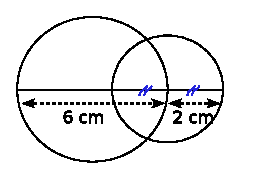
\includegraphics[width=3.4cm]{double-cercle} \end{center}
\end{exercice}


%%%%%%%%%%%%%%%%%%%%%%%%%%%%%%%%%%%Mise en page

\vspace*{3cm}

\phantom{coucou}

\pagebreak
%%%%%%%%%%%%%%%%%%%%%%%%%%%%%%%%%%%%%%%%%%%%%%



\begin{exercice}
Construis chaque figure ci-dessous donnée par son croquis.
\begin{colenumerate}{2}
 \item
 
 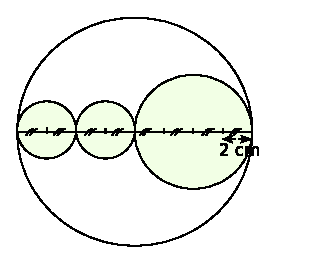
\includegraphics[width=3.9cm]{4cercles}
 \item
 
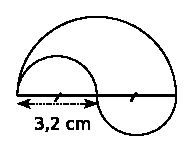
\includegraphics[width=2.6cm]{goutte-rose}
 \item
 
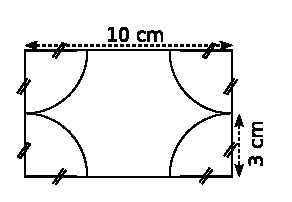
\includegraphics[width=4cm]{theatre}
 \end{colenumerate}
\end{exercice}


\begin{exercice}
En utilisant le quadrillage de ton cahier, reproduis les figures suivantes.
\begin{colenumerate}{2}
 \item
 
 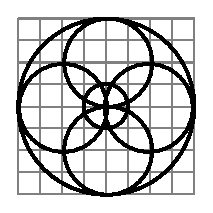
\includegraphics[width=2.9cm]{quadrillage-cercles}
 \item
 
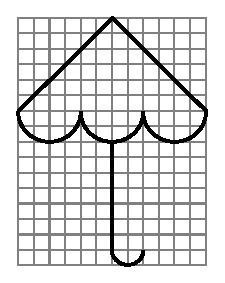
\includegraphics[width=3.1cm]{quadrillage-parap}

 \end{colenumerate}
\end{exercice}


\begin{exercice}[À construire]
\begin{enumerate}
 \item Trace un segment $[AB]$ de longueur 6 cm ;
 \item Marque le point $O$, milieu du segment $[AB]$ ;
 \item Trace le cercle de centre $O$ et de rayon 3 cm ;
 \item Trace les cercles de diamètres $[AO]$ et $[OB]$.
 \end{enumerate}
\end{exercice}



%%%%%%%%%%%%%%%%%%%%%%%%%%%%%%%%%%%Mise en page
\columnbreak
%%%%%%%%%%%%%%%%%%%%%%%%%%%%%%%%%%%%%%%%%%%%%%


\begin{exercice}[À construire (bis)]
\begin{enumerate}
 \item Trace un segment $[AB]$ de longueur 9 cm ;
 \item Trace le cercle de centre $A$ et de rayon 3 cm. On appelle $C$ le point d'intersection de ce cercle et du segment $[AB]$ ;
 \item Trace le cercle de centre $B$ et de rayon 3 cm. Il coupe le segment $[AB]$ en $D$ ;
 \item Trace un demi‑cercle de diamètre $[CD]$.
 \end{enumerate}
\end{exercice}


\begin{exercice}
Complète le programme de construction de la figure ci‑dessous :
\begin{center}  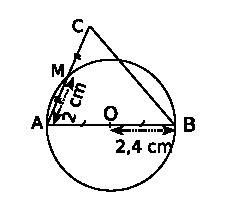
\includegraphics[width=3.6cm]{cercle-triangle} \end{center}
\begin{itemize}
 \item Trace un cercle de \dotfill $O$ et de \dotfill 2,4 cm ;
\vspace{.4em}
 \item Trace un \dotfill $[AB]$ de ce cercle ;
\vspace{.4em}
 \item Trace une \dotfill $[AM]$ telle que $AM =$  \dotfill ;
\vspace{.4em}
 \item Place le point $C$ tel que $M$ soit le  \dotfill de $[AC]$ ;
\vspace{.4em}
 \item Trace le  \dotfill $[CB]$.
 \end{itemize}
\end{exercice}


\begin{exercice}
Écris un programme de construction pour chacune des figures suivantes :

\begin{colenumerate}{1}
 \item 
 \begin{center}
 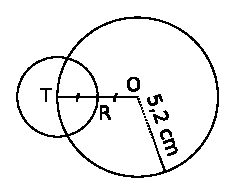
\includegraphics[width=3cm]{double-cercle2}
 \end{center}
 \item 
\begin{center}
\includegraphics[width=5cm]{cercle-triangle2}
\end{center}
 \end{colenumerate}
\end{exercice}







